The \texttt{api} package contains a collection of interfaces for the \texttt{\pkglnk{view.webui.component}} package.

%TODO hier hätte mal ein schöner Abschnitt zur Entkopplung oder Abstraktionsebene hinkommen können
%TODO aber das ist schon lang geschmolzener Schnee von Gestern :(
The interfaces provide consistent naming of methods that the classes for the
\texttt{\pkglnk{view.webui.components}} package implement. This is especially important for
the adapter classes from the \texttt{\pkglnk{view.webui.components}} package.

This layer of abstraction allows to group methods with the same intent that are performed on
various components. This makes it easier to work with a collection of components.

\begin{figure}[H]
	\centering
	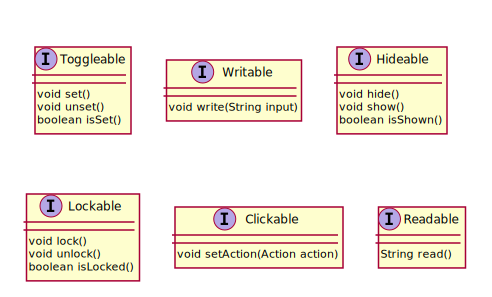
\includegraphics[width=\textwidth]{packageDiagrams/apiPackage}
\end{figure}
